\subsubsection{Physical to logical storage}
\begin{wrapfigure}[14]{r}[0cm]{0.3\textwidth}
    \begin{center}
        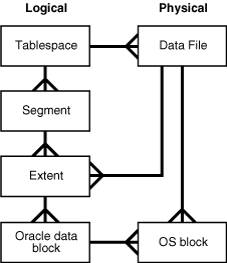
\includegraphics[width=0.25\columnwidth]{assets/db-system-entity-relationship.png}
    \end{center}
    \caption{Entity relationship diagram, where the crow's feet imply one-to-many relationships
        (Figure from \hlhref{https://docs.oracle.com/en/database/oracle/oracle-database/19/cncpt/img/cncpt227.gif}{Oracle Docs})}
    \label{fig:entity-relation-diagram}
\end{wrapfigure}

To the left, in figure \ref{fig:entity-relation-diagram}, the relationship between the different storage
abstractions are connected using crow's feet.

Since database tables often include large amounts of data, that would span many OS pages, thus database systems use blocks as opposed to OS pages.


These database blocks are structured as follows:
\begin{itemize}
    \item \bi{Header}: Contains the address and type of segment (that being index, table, etc)
    \item \bi{Table directory}: Contains the schema of the table stored in the block
    \item \bi{Row directory}: Contains pointers to the actual tuples stored in the block. Grows downwards (like the stack)
    \item \bi{Free Space}: Well... it's free real estate, isn't it?
    \item \bi{Row data}: The tuples stored in the block. Grows upwards (like the heap).
          The pointers in the row directory point here
\end{itemize}

Typically, database systems allow inserts of new tuples until there is about 20\% of free space left.
This space is allocated to allow for updates of existing tuples, as they may become larger.
Thus, a larger storage footprint is used to prevent having to move all the data to a different location when the data block inevitably fills up,
avoiding thrashing on the page.

Some systems even go a step further, only again unlocking a data block for writing if its used percentage falls below 40\%.

Of course, as with any storage system, fragmentation becomes an issue.
Compaction is only done when the block has enough space for an \texttt{INSERT} or \texttt{UPDATE}, but the space is not contiguous.

An \texttt{UPDATE} may require that a tuple is moved into a different block. In that case, the tuple is inserted into a new block and a pointer is stored in the freed space.
